\chapter{Theory}

This section will consider the Danish Healthcare System history and structure. Denmark is a welfare state and therefore a bit different from other western countries. Moreover this chapter will provide a view on the rehabilitation process of cardiac patient and the use of ICT in telemedicine.

\section{The Danish Healthcare System} \label{DHS}

The establishment of the Danish Healthcare System started in the eighteenth century. The first hospital was placed in Copenhagen and opened in 1757. This hospital is still running and today it is known as "Rigshospitalet". Outside of the capital small hospitals were built during the late eighteenth century. At that time the hospitals were partly financed by taxes, patient payment and charity. In the late nineteenth century every thirteenth Dane was a member of a sick-benefit association which the Danish Government co-funded. The Danish Welfare State has roots in 1933 where The Social Reform was founded. By this reform, to all Danes with a low income it became a demand that they were members of a sick-benefit association. During the thirties taxes gradually became the dominant finance source at the Danish Healthcare System \cite{sundhedsvaesen}. 

The sick-benefit associations were shut down in 1973 and replaced by a public health insurance. The Danish public health insurance is paid by Danes themselves from taxes. The insurance provides free care for everyone regardless of income and residence. This public health insurance includes hospital stays, surgery, visits to a General Practitioner (GP) and specialist'. Furthermore, it provides partly funding for dentist, physiotherapist, chiropractor, podiatrist and contributes to medicine \cite{rasmussen2011hjerterehabilitering, Healthcareindk2}.

\subsubsection{Structure of the Danish Healthcare System}
Every healthcare system consists of users, healthcare institutions and the financial third part. Apart from that there are three fundamental financial mechanisms; user fee, tax and budgets/rates. These three financial mechanisms links together the Danish Healthcare System. This is described with the tripartite model in \cref{Trepartmodel}. A, B and C is the financial mechanism and 1, 2 and 3 are the components within the healthcare system. The model shows how a third part is pushed in between users and healthcare institutions. This third part creates equality between users as much as possible. The constellation of finances differs from country to country. Denmark is mostly funded by the Government through taxes whereas US citizen needs health insurance to pay for these services \cite{sundhedsvaesen}. 


\begin{figure}[H]
\centering
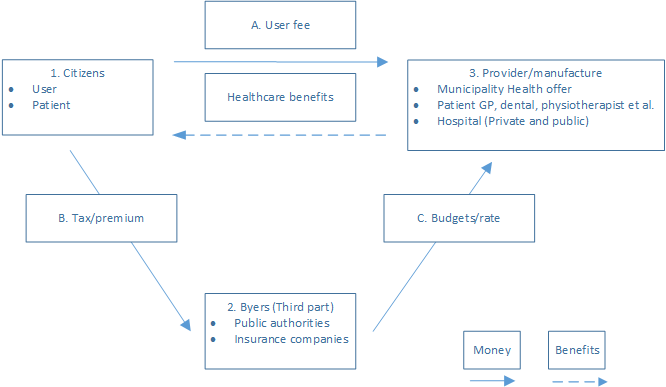
\includegraphics[width=1\textwidth]{Figure/thirdpart.png}
\caption{Tripartite model \cite{sundhedsvaesen}}
\label{Trepartmodel}
\end{figure} 

In 1927 there was a total of 160 somatic hospitals in Denmark. Today the Danish Health Authority is responsible for planning the distribution of specialized hospitals. The Danish Healthcare Authority made a decision to centralize hospitals to improve quality and efficient use of resources. This concerns both acute, long-term and psychiatric care sectors.
The centralization leads to a structural change within the hospitals. Small hospitals got shut down and big hospitals have been modernized. Besides these alterations seven new greenfield projects are under construction. These projects are specialized hospitals. The new hospital construction requires modernized technology and new solutions to ensure cost effective care and shorter admission time \cite{Healthcareindk2}. 

The average length of the admission has decreased with 40\%, which makes Denmark the country with shortest length of hospital stay in Scandinavia. The decline is due to more effective treatments and outpatient treatments. The Ministry of Health is constantly seeking to improve the sector both in quality and efficiency at a minimum cost. Hereby the ministry set up some future goals and one of them is to minimize bed days. "As a result of the modernisation process, the number of bed days is expected to be reduced by 20 percent, and outpatient treatment to be expanded by 50 percent from 2007 to 2020". To manage greater distance between both hospitals and patients, ICT solutions will be a major factor in the development of communication within the new hospital construction\cite{DKhealthreview, Healthcareindk2}. 

In 2007 the Danish State made big structural changes throughout the healthcare organisation. Municipalities were combined which meant a change from 275 municipalities down to 98. The 14 counties were replaced by five regions. The Danish Healthcare System was thereby organized in three levels: State (national level), region (regional level) and municipalities (local level) \cite{indenrigs, Healthcareindk2}.\\

The municipalities have multiple tasks but in the health area they administrate GP's, home nursing, public healthcare, school health service, child dental treatment, prevention and rehabilitation\cite{sundhedsministeriet}. \\

The five regions are responsible for the secondary sector which is mainly focusing on the hospital sector. Each region is able to organize their services accordingly to their regional needs. They may adjust within the national legal limits, but the region will be responsible of procurement of staff and equipment.\\

The states task is to initiate, coordinate, and advise. Furthermore, the job is to establish goals for the national health policy \cite{sundhedsministeriet}. In Denmark a ministry takes care of this job. The ministry changes over time but in 2015 the name of the ministry became Ministry of Health \cite{ministryofhealth}. This ministry is responsible for establishing the overall framework for the provision of health and elderly care.


\subsubsection{Finances}

The region is financed by four subsidies: Block grant from the state (75\%), state activity-related subsidy (5\%), local contribution (10\%) and local activity-related contribution (10\%). The block grant from the state is distributed with the consideration of differences inside the regions which will give the regions equal prospect of providing healthcare services. The rest of the subsidies are divided in three different types of distribution, this is partly to encourage the regions and municipalities to increase activity and efficiency \cite{sundhedsministeriet}.

The municipalities are financed with a block grant from the state but also council taxes which differs in the municipalities. The regions receive activity-based subsidy from the municipality which means that the municipality pays the region money depending on the number of hospitalisations and treatments performed at the hospital. Due to this constellation the municipality has incitement to reduce demands for hospitalization and other regional healthcare services \cite{Healthcareindk2}.

The finance structure in the Danish Healthcare System aims to strengthen health clinical production and responsiveness with free choice of hospital in combination with the activity-based financing. Throughout the structure plan in 2007 the municipalities where given a financial incentive to keep their citizens healthy \cite{DKhealthreview}.

\subsubsection{Preventive healthcare}

As a part of the local government reform in 2007 preventive healthcare became an important part of the Danish Healthcare System. The vision was to improve quality of life and impact the lifestyle related diseases like cancer and cardiovascular diseases which are the dominant cause of mortality today in Denmark. Furthermore, it included focus on risk factors as tobacco, alcohol and lack of exercise. The municipalities were given the primary responsibility for preventive health \cite{sundhedsministeriet}.

\subsubsection{Rehabilitation}

Rehabilitation, including both physical and mental training programmes, are offered to all citizens by the municipalities. Training and rehabilitation of a patient may be initiated at the hospital and continued within the municipality when the patient is discharged. This means that the municipality will be responsible for the rehabilitation after discharge. Rehabilitation helps the patient to regain functional abilities and helps them to become self-sufficient. Some patients will receive rehabilitation free of charge whereas others may pay partly by themselves. This depends on type of illness \cite{Healthcareindk2, retningsrehab, WHO}.


\subsubsection{Treatment of Cardiac patients}

In 2010 treatment packages for non-acute heart disease were introduced in Denmark. This package included a process consisting of investigation, diagnosis, treatment and rehabilitation. The Danish Health Authority decided to phase out the package deal in 2017. With the new alteration the patient will achieve a more simple and coherent treatment with better quality. 
The progress for the patient is divided in five steps and will be described in the next section. \\

\textbf{Step 1} Preliminary assessment and referral: When a patient feels ill they contact their GP, unless it is acute. It is the GP's job to carry out preliminary examination and to give the patient the right kind of treatment if necessary. The GP should include the patient in choice of treatment plan and decide if the patient needs to be admitted to the hospital or an outpatient treatment is necessary. 
\newline
\newline
\textbf{Step 2} Investigation and treatment: The investigation and treatment of cardiovascular patients differs from different diagnoses. Common is, that the knowledge of comorbidity is important due to stabilization and treatment of the concurrent disease throughout the treatment of the cardiovascular disease. The health facility will form a treatment plan in corporation with the patient. 
\newline
\newline
\textbf{Step 3} Planning follow-up on treatment, rehabilitation and palliation: At the end of treatment the cardiology department/specialist practice performs a systematic assessment of needs. The needs assessment is carried out in collaboration with the patient and perhaps relatives. 
\newline
\newline
\textbf{Step 4} Follow-up: When the patient has been discharged from the hospital the treatment will pursue as outpatient visits while others will pursue follow-up at their GP's. 
\newline
\newline
\textbf{Step 5} Rehabilitation and palliation: Patients with heart disease should systematically perform a need assessment in order to offer rehabilitation and palliative action based on patient needs and heart disease. Rehabilitation with cardiac patients is mainly performed with focus on disease coping, nutrition, physical training, tobacco cessation and work retention. Furthermore, it aims to improve the individuals physical and mental state of health. The rehabilitation is primarily placed in the municipalities. The effort of rehabilitation planning should origin in the patients functioning, preferences and resources. Motivation, participation and adherence of achieved change of behaviour are important elements in the rehabilitation process. After a heart disease the patient is at great risk of developing anxiety and depression and it is therefore important that physicians related to the rehabilitation process are observant. 
\newline
\newline
Patients with heart disease experience varying periods of worsening of the disease along with more calm periods. In connection with impairments and possible subsequent hospitalization, there will often be uncertainty as to whether the patient survives. This is always a burden for both the patient and the relatives. In this regard, it is important for health professionals to pay attention and to assess the patient's and their dependents' palliative needs and problems associated with heart disease. It is important that the need is assessed on a regular basis to prevent efforts from initiating too late \cite{behandlingsforlob}.


\section{ICT in telemedicine}

The first use of telemedicine was in 1877. A group of doctors made a communication network towards the drug store by using telephones. The first video consultation between a doctor and a patient took place in 1927. In the 1950s a two way television group therapy took place in Alaska. In the 1970s NASA built \textit{Space Technology Applied to Rural Papago Advanced Health Care (STARPAHC)}. By this system they were able to communicate with a two-way radio and to deliver and send data. It was not until the eighties where the technology had renewed interest, due to high cost, lack of suitable technologies and unacceptance. At this point the military picked up the idea of the usage of telemedicine in combat. The use of technology in military has extended to hospitals throughout the world. 

Telemedicine is a generic term that covers different types of healthcare which is provided digitally and in distance. Telemedicine range from tele consultations to telesurgery. Telemedicine has made it possible to give specialized care and diagnostic medicine for people in rural and remote areas. The introduction of telemedicine has changed the traditional doctor-patient relationship. 

ICT is an information and communication technology which allow people to interact in the digital world. Telemedicine uses ICT as the digital communaction method. ICT has drastically changed the way the world in general communicates, work, learn and live. The use of ICT in telemedicine has made cost-effective treatment options available due to reduced traveling expenses, decreasing hospital readmission rates, and maximization of consultations. It is important to keep in mind, that providing medical care with the use of telemedicine opens important medical, ethical and legal issues, which must be addressed and considered \cite{considerations}.


